\chapter{Arhitektura i dizajn sustava}

		\textit{ Arhitektura ima 3 podsustava:}
	\begin{itemize}
		\item 	\textit{Web preglednik}
		\item 	\textit{Web aplikacija na web poslužitelju}
		\item 	\textit{Baza podataka - PostgreSQL }		
	\end{itemize}


{\underline{Web preglednik} je ujedino i prevoditelj koda koji korisniku omogućuje pregledavanje sadržaja web aplikacije i interakciju s istim.}

{\underline{Web poslužitelj} prima HTTP (engl. Hyper
Text Transfer Protocol) zahtjeve od klijenta (preglednika) koji sadrže informacije o tome što klijent traži, kao što su primjerice URL, GET, POST... i vraća dohvaćeni resurs ako ga ima te vraća statusni kod koji daje informacije o uspješnosti zahtjeva.}

{Tehnologije korištene u našoj aplikaciji jesu Spring Boot i React. Aplikacija se sastoji od serverske komponente napisane u Javi (Spring Boot) i klijentske komponente napisane u JavaScriptu (React). Za razvojno okruženje koristimo IntelliJ, a baza koju koristimo za spremanje podataka o registriranim korisnicima i sve informacije o natjecanjima je PostgreSQL.}

{\underline{Web aplikacija} temelji se na arhitekturi Model-View-Controller (MVC). Ova arhitektura omogućuje organizaciju aplikacije u tri ključne komponente:}

\begin{itemize}
    \item \textbf{Model}: Ova komponenta predstavlja poslovnu logiku i podatke aplikacije. Model je implementiran u Java programskom jeziku (Spring Boot) i odgovoran je za upravljanje podacima, komunikaciju s bazom podataka te izračune i obrade podataka.
    
    \item \textbf{View}: Komponenta za prikaz podataka korisnicima. Prikazi se generiraju u Reactu, a omogućuju korisnicima interakciju s aplikacijom putem web preglednika. Prikazi se oblikuju pomoću HTML-a, CSS-a i JavaScripta.
    
    \item \textbf{Controller}: Kontroler je posrednik između Modela i Viewa. Ova komponenta upravlja korisničkim zahtjevima, prima ulazne podatke od korisnika te izvršava odgovarajuće akcije u Modelu. Kontroler također određuje koji prikaz treba biti poslan korisnicima.\\
\end{itemize}	

				
		\section{Baza podataka}
			

			
		{Koristimo relacijsku bazu podataka čije su gradivne jedinke tablice definirane imenom i skupom atributa za jednostavno upravljanje podacima. Baza podataka ove aplikacije sastoji se od sljedećih entiteta:}
	\begin{itemize}
		\item 	\textit{Korisnik}
		\item 	\textit{Natjecanje}
		\item 	\textit{Zadatak}
		\item 	\textit{Zadaci na natjecanju}
		\item 	\textit{Primjeri za evaluaciju}	
		\item 	\textit{Slike}		
	\end{itemize}
		
			\subsection{Opis tablica}
			

				{\textbf{Korisnik} - entitet sadržava sve važne informacije o korisniku: Korisničko ime, lozinku, ime, prezime, identifikator slike, email, tip korisnika (natjecatelj/voditelj), individualni sažetak, potvrda registracije, potvrda administratora. U vezi je One-To-One sa entitetom slika }
				
				
				\begin{longtblr}[
					label=none,
					entry=none
					]{
						width = \textwidth,
						colspec={|X[6,l]|X[6, l]|X[20, l]|}, 
						rowhead = 1,
					} %definicija širine tablice, širine stupaca, poravnanje i broja redaka naslova tablice
					\hline \SetCell[c=3]{c}{\textbf{Korisnik}}	 \\ \hline[3pt]
					 \SetCell{LightGreen}id & INT	&   jedinstveni identifikator korisnika	\\ \hline
					 \SetCell{LightBlue} username	& VARCHAR &   	izabrano korisničko ime\\ \hline 
					 \SetCell{LightBlue}email & VARCHAR &  e-mail adresa korisnika \\ \hline 
					 \SetCell{LightBlue}image-id & INT	&  	identifikator slike korisnika	\\ \hline
					 \SetCell{LightBlue}confirmation-hash & VARCHAR & individualni kod za registraciju \\ \hline
					 name & VARCHAR	&  	ime korisnika	\\ \hline 
					 lastname & VARCHAR	&  	prezime korisnika	\\ \hline 										
					 user-type & VARCHAR & natjecatelj ili voditelj natjecanja \\ \hline
					 password & VARCHAR	&  	šifra korisnika	\\ \hline 					 
					 confirmed & BOOLEAN & potvrđena registracija preko korisničkog emaila \\ \hline
					 confirmed-by-admin & BOOLEAN & potvrđena registracija od strane administratora \\ \hline
					   
				\end{longtblr}


				{\textbf{Natjecanje} - entitet sadržava sve važne informacije o natjecanju: Id natjecanja, vrijeme početka, vrijeme završetka, broj zadataka, id voditelja natjecanja, identifikator pehara, ime natjecanja i je li virtualno. U odnosu je Many-To-One s entitetom korisnik preko atributa voditelja natjecanja,  u vezi je One-To-One sa entitetom slika. }
				
				
				\begin{longtblr}[
					label=none,
					entry=none
					]{
						width = \textwidth,
						colspec={|X[6,l]|X[6, l]|X[20, l]|}, 
						rowhead = 1,
					} %definicija širine tablice, širine stupaca, poravnanje i broja redaka naslova tablice
					\hline \SetCell[c=3]{c}{\textbf{Natjecanje}}	 \\ \hline[3pt]
					 \SetCell{LightGreen}id & INT	&   jedinstveni identifikator natjecanja	\\ \hline
					 \SetCell{LightBlue}image-id & INT	&  	identifikator slike pehara	\\ \hline
					  date-time-of-beginning	& TIMESTAMP &   vrijeme početka natjecanja	\\ \hline 
					 date-time-of-ending	& TIMESTAMP &   vrijeme završetka natjecanja	\\ \hline  
					 competition-maker-id & INT	&  	id voditelja natjecanja	\\ \hline 
	 				number-of-problems & INT	&  	broj zadataka u natjecanju	\\ \hline 
	 				name & VARCHAR & ime natjecanja \\ \hline
	 				isVirtual & BOOLEAN & virtualno natjecanja \\ \hline
				\end{longtblr}

				{\textbf{Zadatak} - entitet sadržava sve važne informacije o zadatku. Sadrži atribute id, trajanje zadatka, booleanski atribut is-private, broj bodova koje je moguće ostvariti, tip problema (težinu zadatka), tekst zadatka, naslov i id korisnika koji je napravio zadatak. S entitetom Korisnik je u odnosu Many-To-One preko atributa problem-maker-id.}
				
		\begin{longtblr}[
					label=none,
					entry=none
					]{
						width = \textwidth,
						colspec={|X[6,l]|X[6, l]|X[20, l]|}, 
						rowhead = 1,
					} %definicija širine tablice, širine stupaca, poravnanje i broja redaka naslova tablice
					\hline \SetCell[c=3]{c}{\textbf{Zadatak}}	 \\ \hline[3pt]
					 \SetCell{LightGreen} id & INT	&   jedinstveni identifikator zadatka	\\ \hline
				  \SetCell{LightBlue}problem-maker-id & INT	& identifikator vlasnika zadatka	\\ \hline 
					 duration &  NUMERIC	& trajanje zadatka	\\ \hline 
					 is-private &  BOOLEAN	& provjerava je li zadatak objavljen	\\ \hline 
					 problem-type &  INT	&  težina zadatka	\\ \hline 
					text &  VARCHAR	& tekst zadatka	\\ \hline 
					 title &  NUMERIC	& naslov zadatka	\\ \hline 
					 points & INT  & broj bodova zadatka \\ \hline

				\end{longtblr}

				{\textbf{Zadaci na natjecanju} - entitet sadržava informacije o tome koje natjecanje ima koje zadatke. Atributi: id natjecanja i id zadatka. On predstavlja vezu Many-To-Many natjecanja i zadatka}

				
				\begin{longtblr}[
					label=none,
					entry=none
					]{
						width = \textwidth,
						colspec={|X[6,l]|X[6, l]|X[20, l]|}, 
						rowhead = 1,
					} %definicija širine tablice, širine stupaca, poravnanje i broja redaka naslova tablice
					\hline \SetCell[c=3]{c}{\textbf{Zadaci na natjecanju}}	 \\ \hline[3pt]
					 \SetCell{LightBlue}competition-id & INT	&    identifikator natjecanja (natjecanje.id)	\\ \hline
					 \SetCell{LightBlue} problem-id & INT	& identifikator zadatka	(problem.id) \\ \hline 
				\end{longtblr} 


				

				{\textbf{Primjeri za evaluaciju} - entitet sadržava id zadatka te vrijednost i ključ, odnosno na ovaj način se mapiraju rješenja zadataka i služi za evaluaciju rješenja korisnika.}

				
				\begin{longtblr}[
					label=none,
					entry=none
					]{
						width = \textwidth,
						colspec={|X[6,l]|X[6, l]|X[20, l]|}, 
						rowhead = 1,
					} %definicija širine tablice, širine stupaca, poravnanje i broja redaka naslova tablice
					\hline \SetCell[c=3]{c}{\textbf{Primjeri za evaluaciju}}	 \\ \hline[3pt]
					 \SetCell{LightGreen}problem-id & INT	&  jedinstveni identifikator zadatka	\\ \hline
					 vrijednost & VARCHAR	&  očekivani izlaz programa  \\ \hline 
					 ključ & VARCHAR	&  ulaz programa \\ \hline 
				\end{longtblr}
				
				{\textbf{Slike} - entitet sadržava id slike te bajt zapis slike. Na ovaj način spremamo slike korisnika i pehara. }
				
				\begin{longtblr}[
					label=none,
					entry=none
					]{
						width = \textwidth,
						colspec={|X[6,l]|X[6, l]|X[20, l]|}, 
						rowhead = 1,
					} %definicija širine tablice, širine stupaca, poravnanje i broja redaka naslova tablice
					\hline \SetCell[c=3]{c}{\textbf{Slike}}	 \\ \hline[3pt]
					\SetCell{LightGreen} id & INT	&  jedinstveni identifikator slike	\\ \hline
					data & BYTEA &  binarni kod slike \\ \hline 

				\end{longtblr}
				{\textbf{Tablica sudionika natjecanja} - entitet sadržava id korisnika i id natjecatelja te informaciju do kada korisnik može rješavati natjecanje. Ova tablica predstavlja Many-To-Many vezu natjecanja i korisnika. }
				
				\begin{longtblr}[
					label=none,
					entry=none
					]{
						width = \textwidth,
						colspec={|X[6,l]|X[6, l]|X[20, l]|}, 
						rowhead = 1,
					} %definicija širine tablice, širine stupaca, poravnanje i broja redaka naslova tablice
					\hline \SetCell[c=3]{c}{\textbf{Tablica sudionika natjecanja}}	 \\ \hline[3pt]
					\SetCell{LightBlue}competition\_id & INT & identifikator natjecanja (natjecanje.id) \\ \hline	
					\SetCell{LightBlue}user\_id & INT & identifikator korisnika \\ \hline
					access\_time & TIMESTAMP & rok završetka rješavanja natjecanja za korisnika\\ \hline			
				
				\end{longtblr}
				
				{\textbf{Rang lista} - entitet sadržava id korisnika i id natjecatelja te korisnikov rang. Ova tablica predstavlja Many-To-Many vezu natjecanja i korisnika. }
				
				\begin{longtblr}[
					label=none,
					entry=none
					]{
						width = \textwidth,
						colspec={|X[6,l]|X[6, l]|X[20, l]|}, 
						rowhead = 1,
					} %definicija širine tablice, širine stupaca, poravnanje i broja redaka naslova tablice
					\hline \SetCell[c=3]{c}{\textbf{Rang lista}}	 \\ \hline[3pt]
					\SetCell{LightGreen} user\_id & INT	& identifikator korisnika \\ \hline
					placement & INT & rang korisnika \\ \hline
					\SetCell{LightGreen}competition\_id & INT & identifikator natjecanja (natjecanje.id) \\ \hline					
				\end{longtblr}
				
				{\textbf{Rezultati natjecanja} - entitet sadržava jedinstven identifikator, id natjecatelja, korisničko ime natjecatelja, i osvojene bodove te korisnikov rang. Ova tablica predstavlja Many-To-Many vezu natjecanja i korisnika. }
				
				\begin{longtblr}[
					label=none,
					entry=none
					]{
						width = \textwidth,
						colspec={|X[6,l]|X[6, l]|X[20, l]|}, 
						rowhead = 1,
					} %definicija širine tablice, širine stupaca, poravnanje i broja redaka naslova tablice
					\hline \SetCell[c=3]{c}{\textbf{Rezultati natjecanja}}	 \\ \hline[3pt]
					\SetCell{LightGreen} id & INT &  jedinstven identifikator	\\ \hline
					points & NUMERIC & osvojeni bodovi\\ \hline 	
					\SetCell{LightBlue}competition\_id & INT & identifikator natjecanja \\ \hline
					\SetCell{LightBlue}username & VARCHAR & korisničko ime\\ \hline
					
				\end{longtblr}
				{\textbf{Učitana programska rješenja} - entitet sadržava jedinstven identifikator, bitove pohranjenog rješenja, vrijeme od početka rješavanja do predaje, korisničko ime, identifikator zadatka, ostvarene bodove, identifikator natjecanja, postotak točnosti i radi li se o virtualnom učitanju. Ova tablica predstavlja Many-To-Many-Many vezu natjecanja, korisnika i zadatka. }
				
				\begin{longtblr}[
					label=none,
					entry=none
					]{
						width = \textwidth,
						colspec={|X[6,l]|X[6, l]|X[20, l]|}, 
						rowhead = 1,
					} %definicija širine tablice, širine stupaca, poravnanje i broja redaka naslova tablice
					\hline \SetCell[c=3]{c}{\textbf{Učitana programska rješenja}}	 \\ \hline[3pt]
					\SetCell{LightGreen} id & INT &  jedinstven identifikator	\\ \hline
					file\_data & BYTEA & binarni kod rješenja  \\ \hline 
					time\_taken & INT & vrijeme od početka rješavanja do predaje \\ \hline
					\SetCell{LightBlue}problem\_id & INT & identifikator zadatka \\ \hline
					\SetCell{LightBlue}username & VARCHAR & izabrano korisničko ime\\ \hline
					points & NUMERIC & ostvareni bodovi\\ \hline
					\SetCell{LightBlue}competition\_id & INT & identifikator natjecanja (natjecanje.id) \\ \hline
					percentage\_of\_
					total & DOUBLE & postotak točnosti \\ \hline
					is\_virtual & BOOLEAN & virtualno učitanje \\ \hline
				\end{longtblr}
				
				
				
			
			\subsection{Dijagram baze podataka}
				
				\noindent {ER dijagram baze podataka prikazan na slici \ref{fig:erdijagram} sadrži vizualne slike ključeva: primarni ključ prikazan je ikonom ključa žute boje, strani ključ sivom bojom, a atributi označeni brojem 1 su alternativni ključevi. Prvi redak svake tablice entiteta predstavlja vidljivost tablice u bazi podataka, u drugom se retku nalazi ime tablice, a u preostalim retcima su ispisani atributi.
				}\\
					\centering
					\begin{figure}[H]
					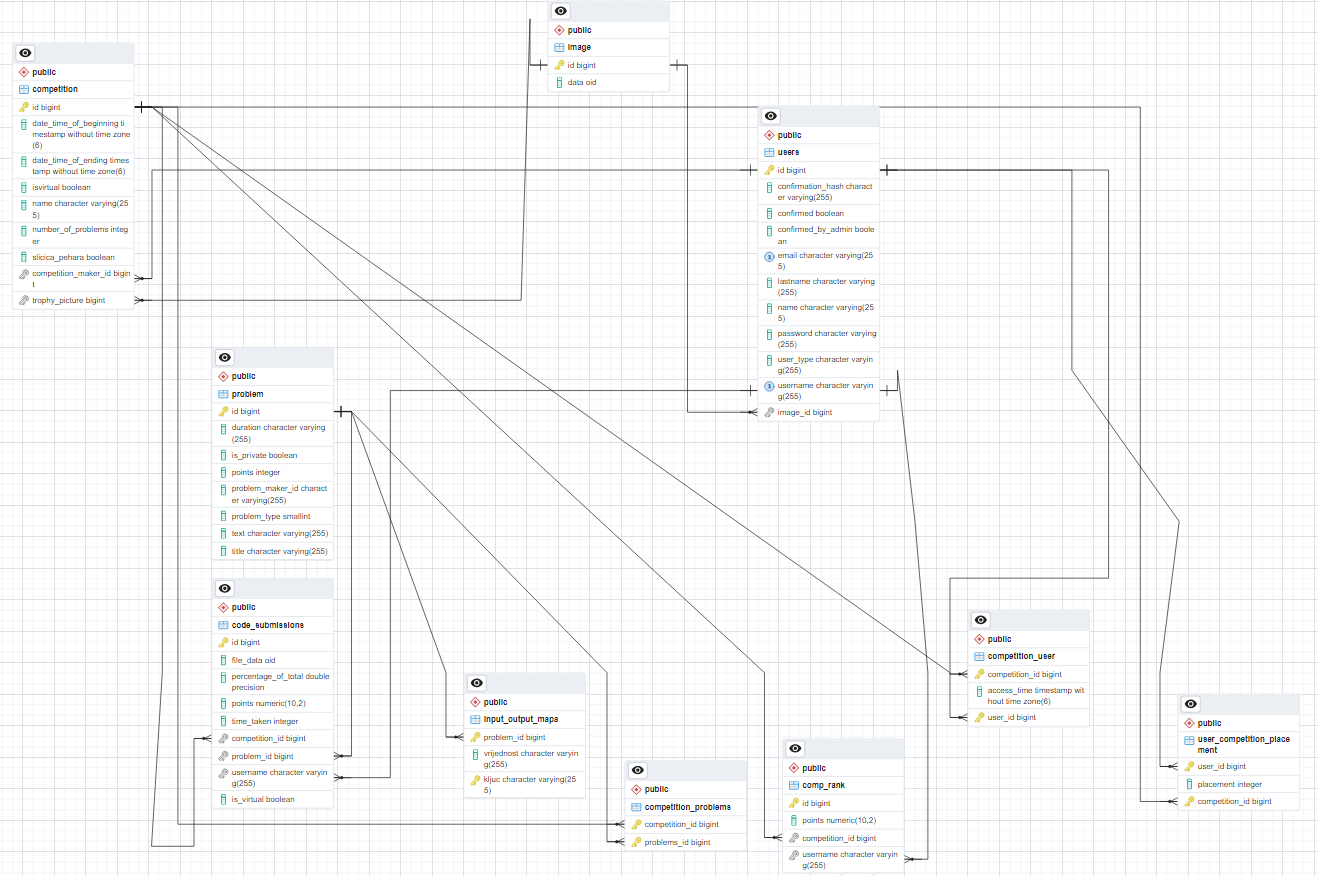
\includegraphics[scale=0.5]{slike/DijagramBa}
					%veličina slike u odnosu na originalnu datoteku i pozicija slike
					\centering
					\caption{Er dijagram baze podataka}
					\label{fig:erdijagram}
				\end{figure}

			
			\eject
			
			
		\section{Dijagram razreda}
		
			\noindent {U nastavku su prikazani razredi na kojima je zasnovan backend aplikacije.
				Lako je uočljivo da većina njih u nazivu sadrži naziv entiteta iz baze, te riječi Service i Controller. 
			}\\
				\begin{figure}[H]
				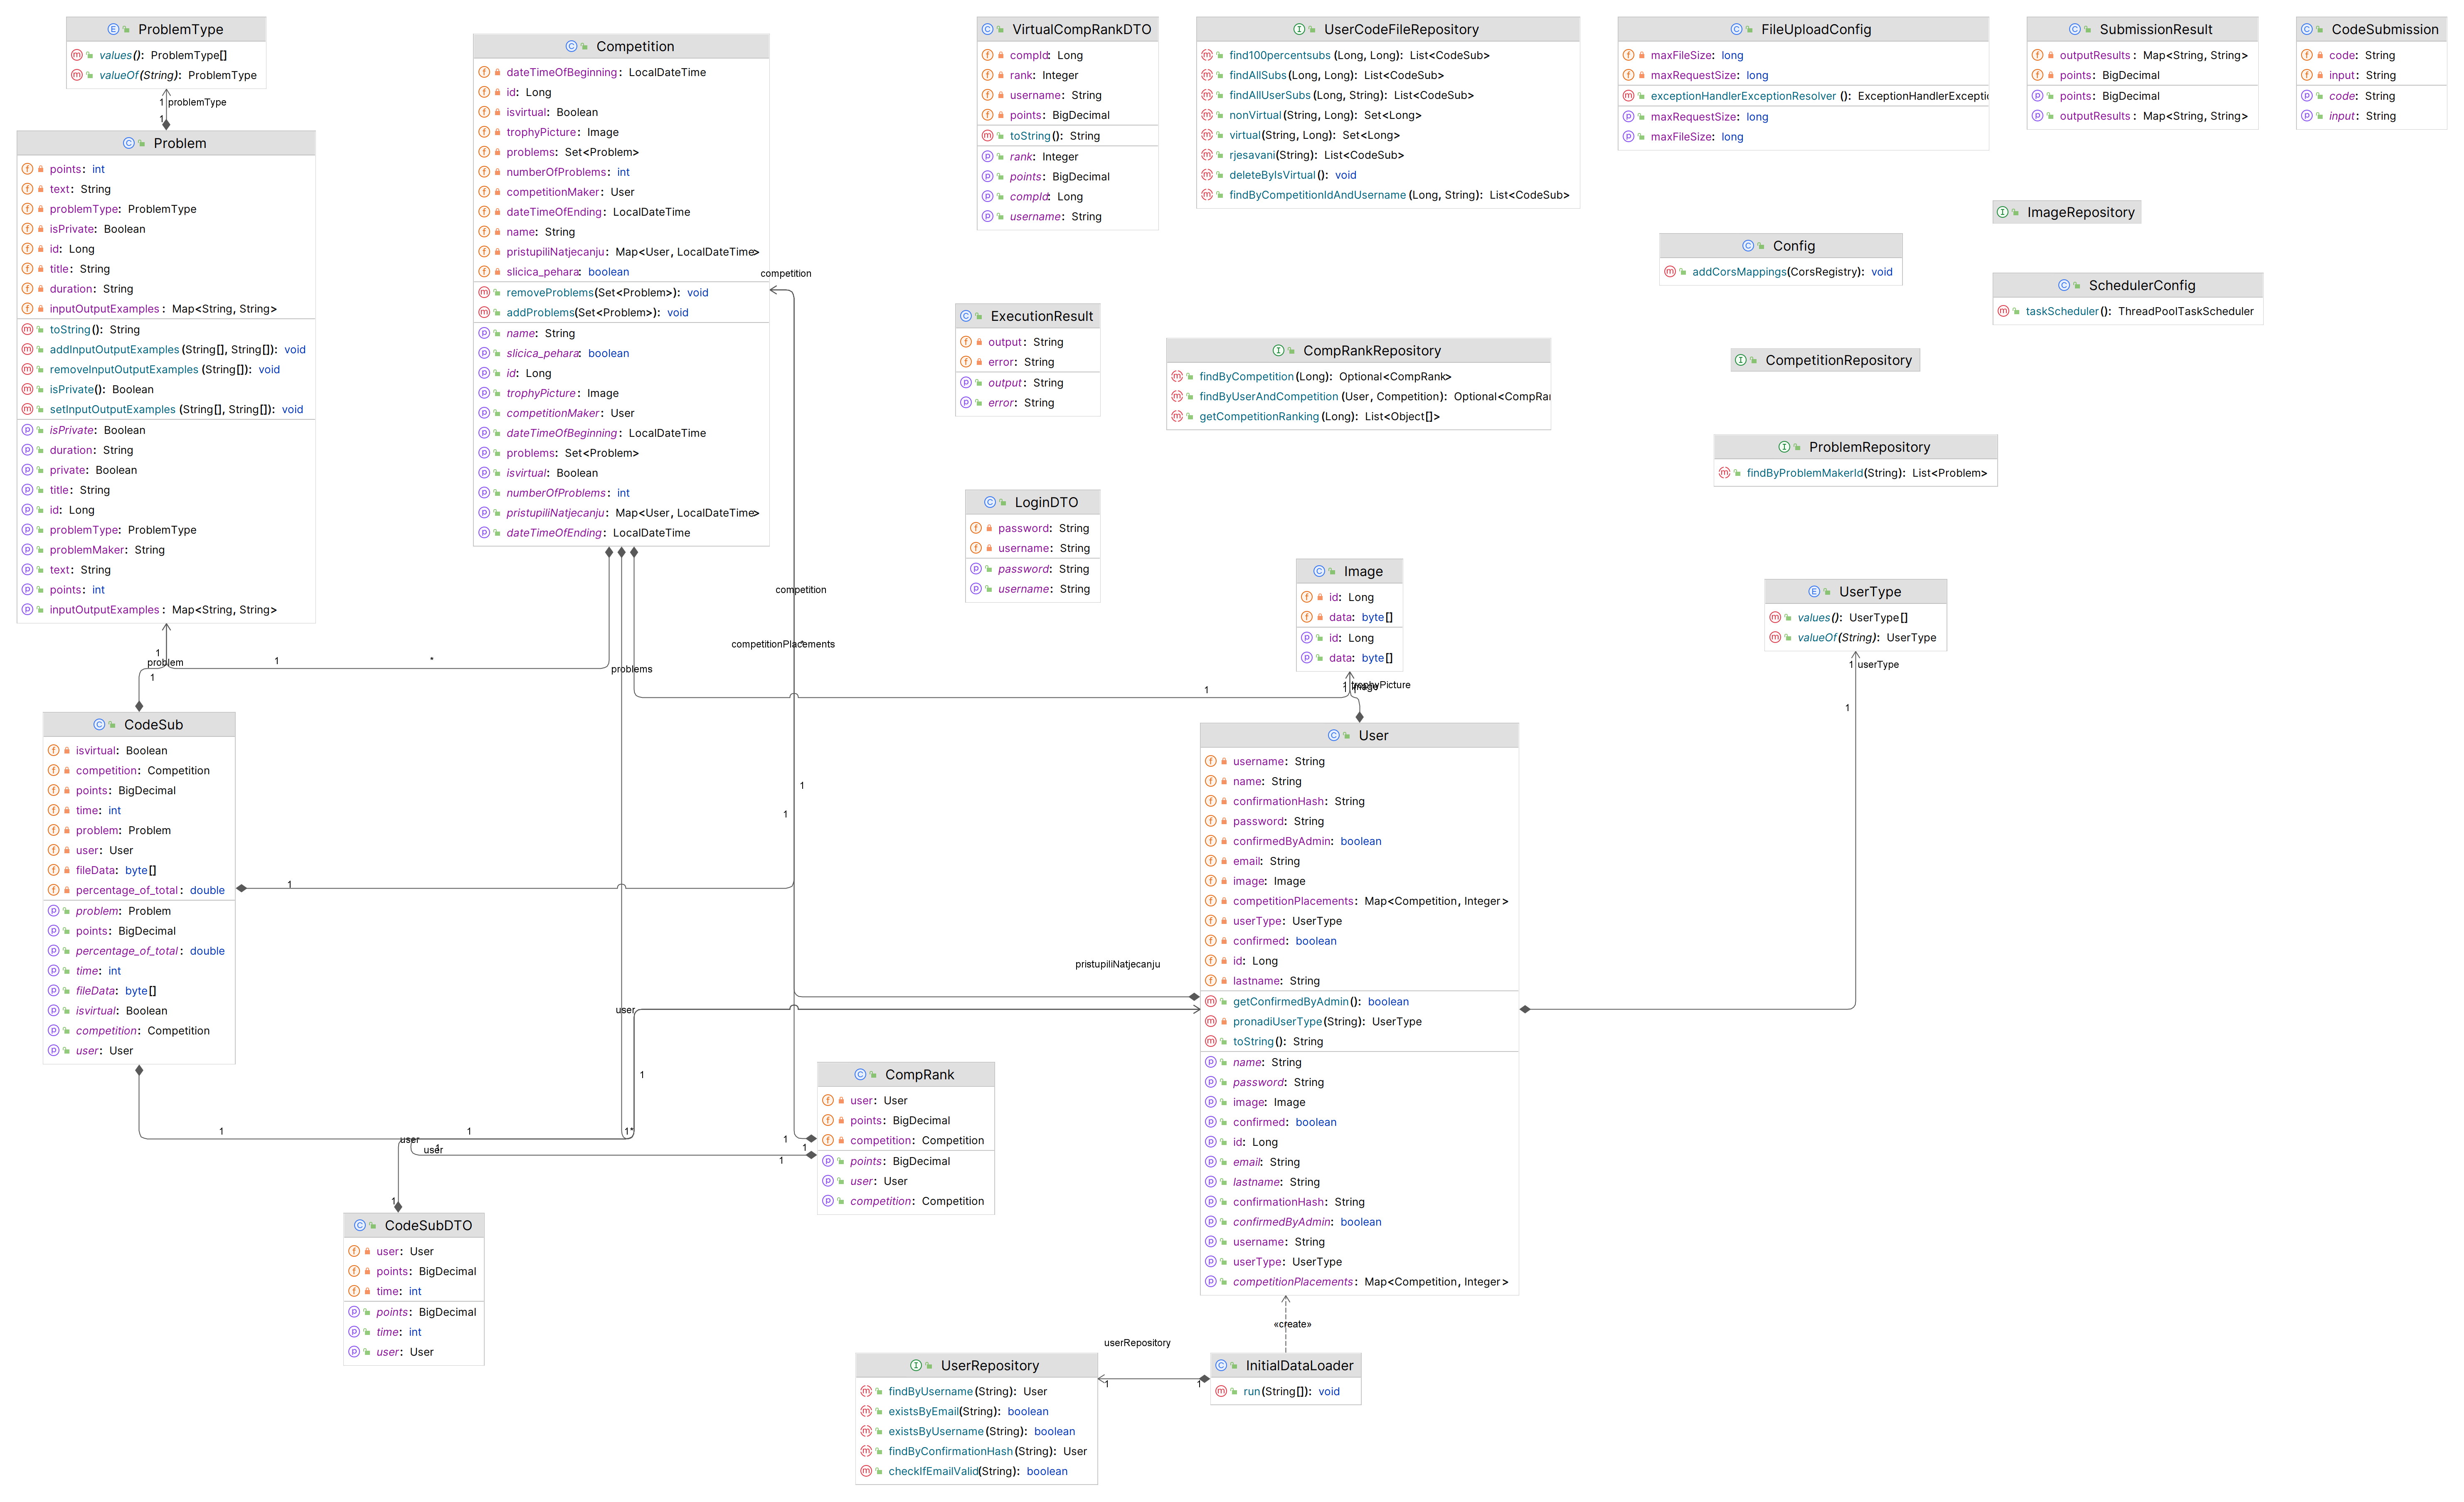
\includegraphics[scale=0.08]{slike/klase}
				%veličina slike u odnosu na originalnu datoteku i pozicija slike
				\centering
				\caption{Dijagram razreda: razredi koji predstavljaju strukturu baze}
				\label{fig:dr2}
			\end{figure}
			
			\noindent{
				 Razredi User, Competition, Image, CodeSub i Problem sa slike \ref{fig:dr2} preslikavaju atribute svakog od entiteta iz baze. Razred User predstavlja registriranog korisnika, čiji UserType može biti COMPETITOR, COMPETITION LEADER i ADMIN (samo jedan, glavni korisnik), a koji pri registraciji unosi podatke prikazane na dijagramu (koji su vlastiti atributi razreda User). Razred Problem predstavlja zadatak koji je korisnik s tipom voditelj unio u sustav: na dijagramu se vidi ta poveznica. Jedna ili više instanci razreda Problem je dio Natjecanja tj. razreda Competition. Jedan korisnik može sudjelovati na više natjecanja, kao što i na jednom natjecanju sudjeluje jedan ili više korisnika. 
				Tu je i razred Image koji služi za pohranu slike u bazu podataka, te razred CodeSub koji prati predaju rješenja zadataka te njihovo bodovanje. 		
					
				Razredi imena Service (slika \ref{fig:dr}) služe za baratanje objektima razreda User, Competition itd. Razredi imena Controller (slika \ref{fig:dr1}) obrađuju HTTP zahtjeve poslane na server i vraćaju zatražene podatke u .json obliku. 	
				
				 Strelice sa slike na jednostavan i intuitivan način prikazuju poveznice između razreda User, UserController i UserService. Metode koje su u razredima implementirane služe za baratanje entitetima u bazi: primarno su to razredi koji u svome nazivu sadrže 'Service' kao što je prije rečeno. Razred UserController oslanja se na ta dva prethodno navedena razreda da bi mogao ispuniti zaprimljene HTTP zahtjeve, bilo da je to samo informacija o korisnicima ili izmjena podataka.
				 
				 Prikazan je i TokenService razred koji omogućava autentifikaciju korisnika, a time sadrži i informacije o njegovim ovlastima u aplikaciji. 
			}\\
			
			
			\begin{figure}
			\centering
			\begin{minipage}[b]{0.45\textwidth}
				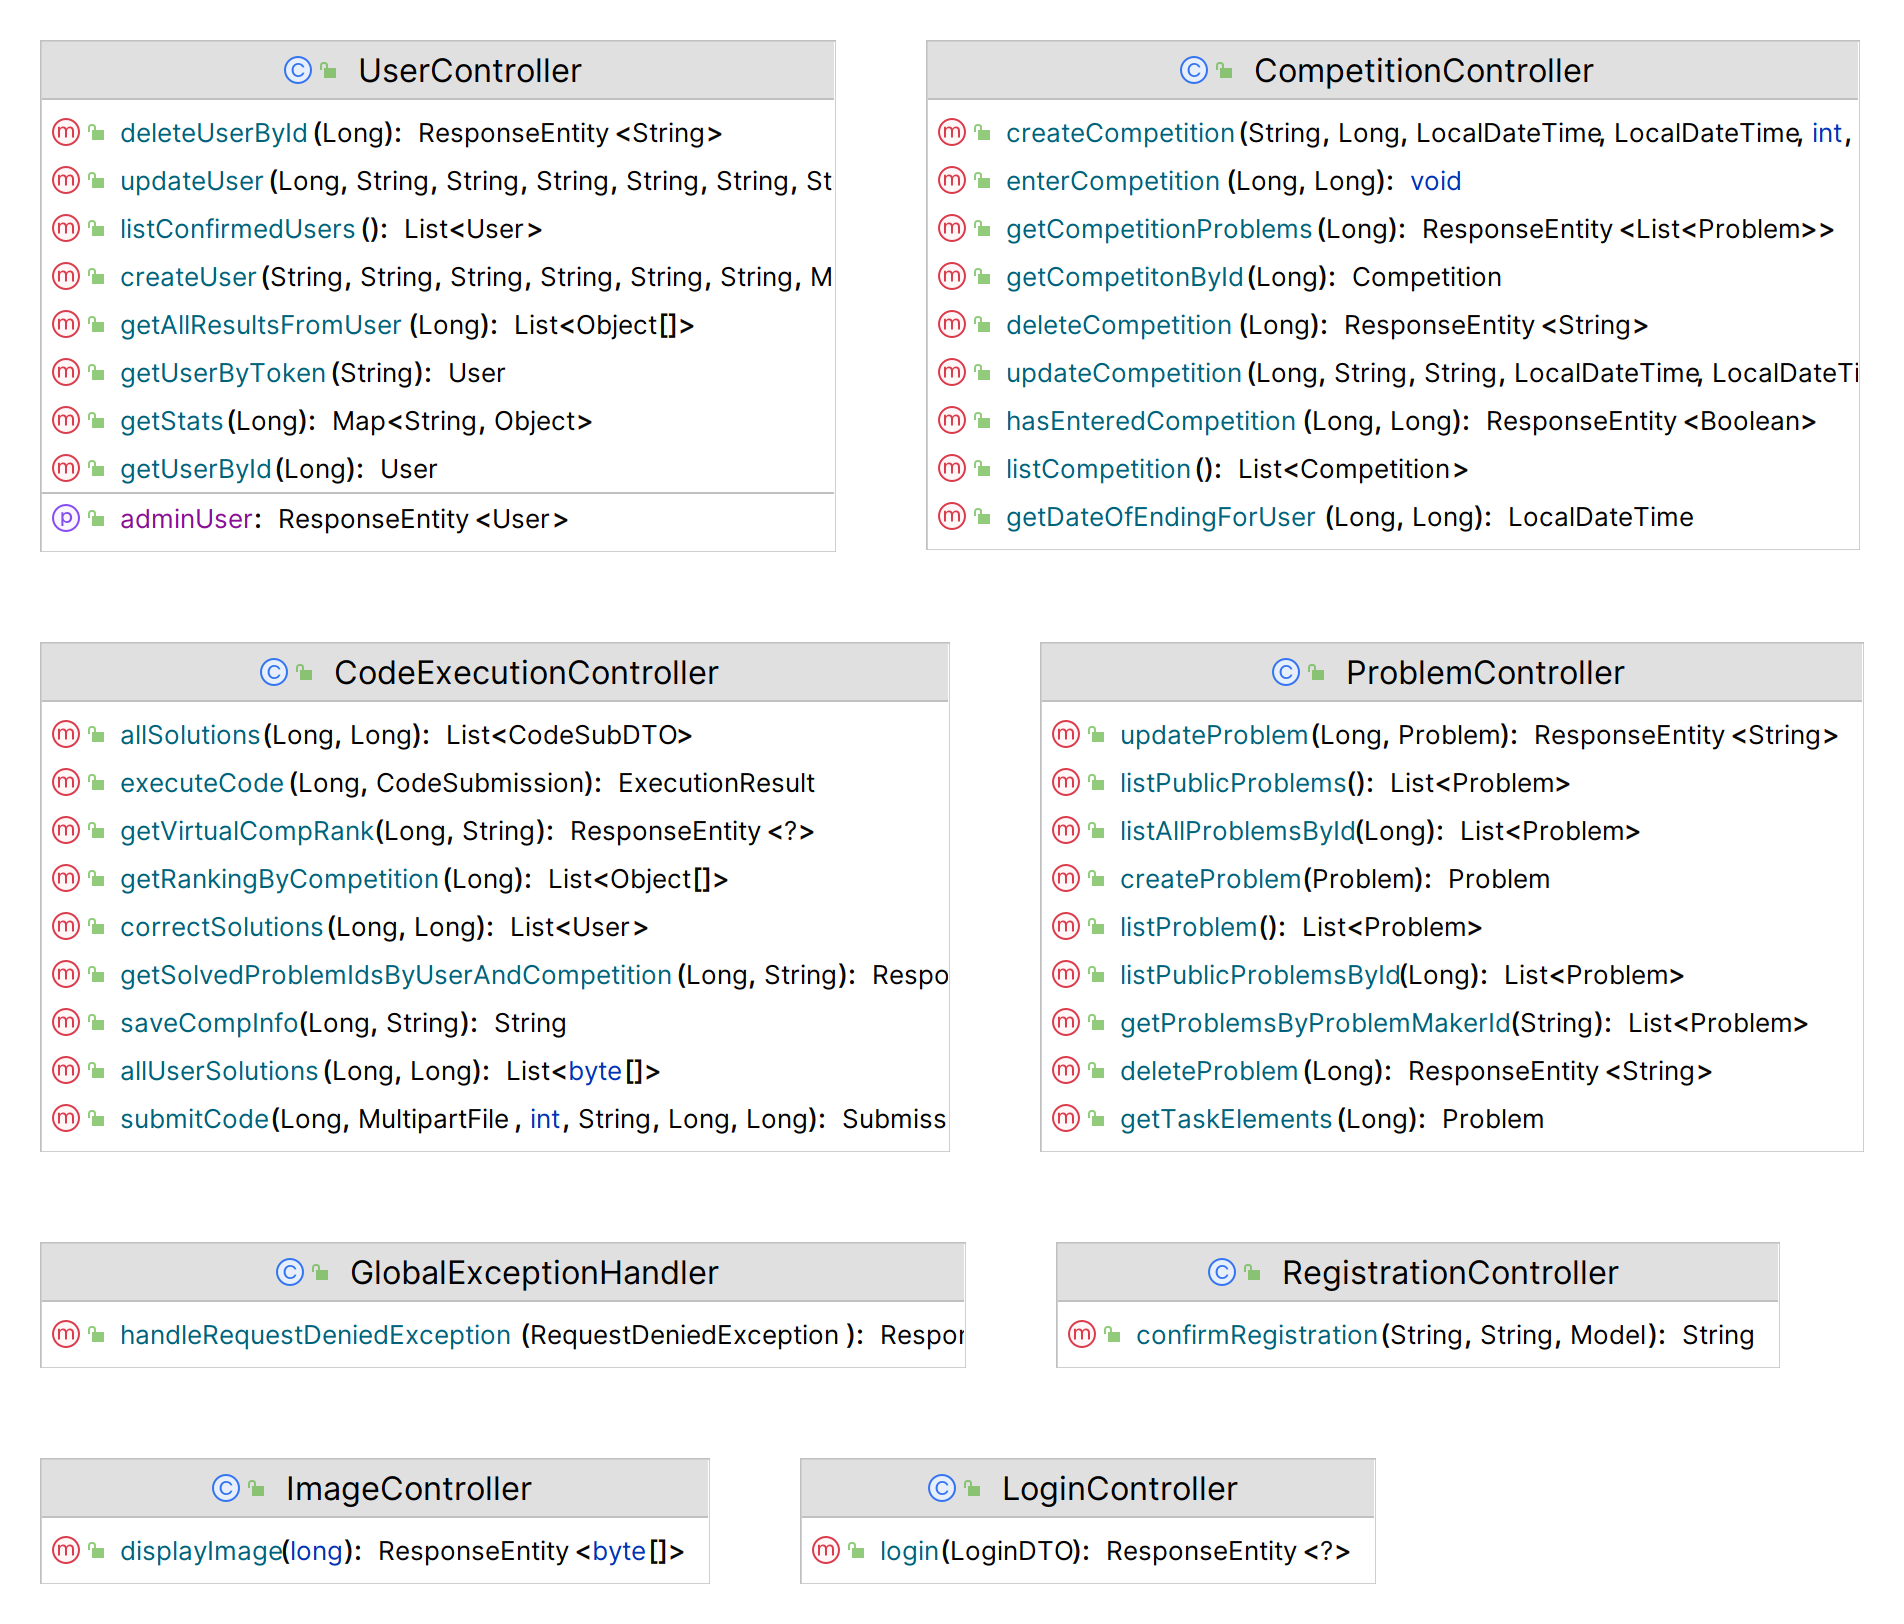
\includegraphics[width=\textwidth]{slike/controlleri}
				\caption{Dijagram razreda: razredi Controller}
				\label{fig:dr1}
			\end{minipage}
			\hfill
			\begin{minipage}[b]{0.45\textwidth}
				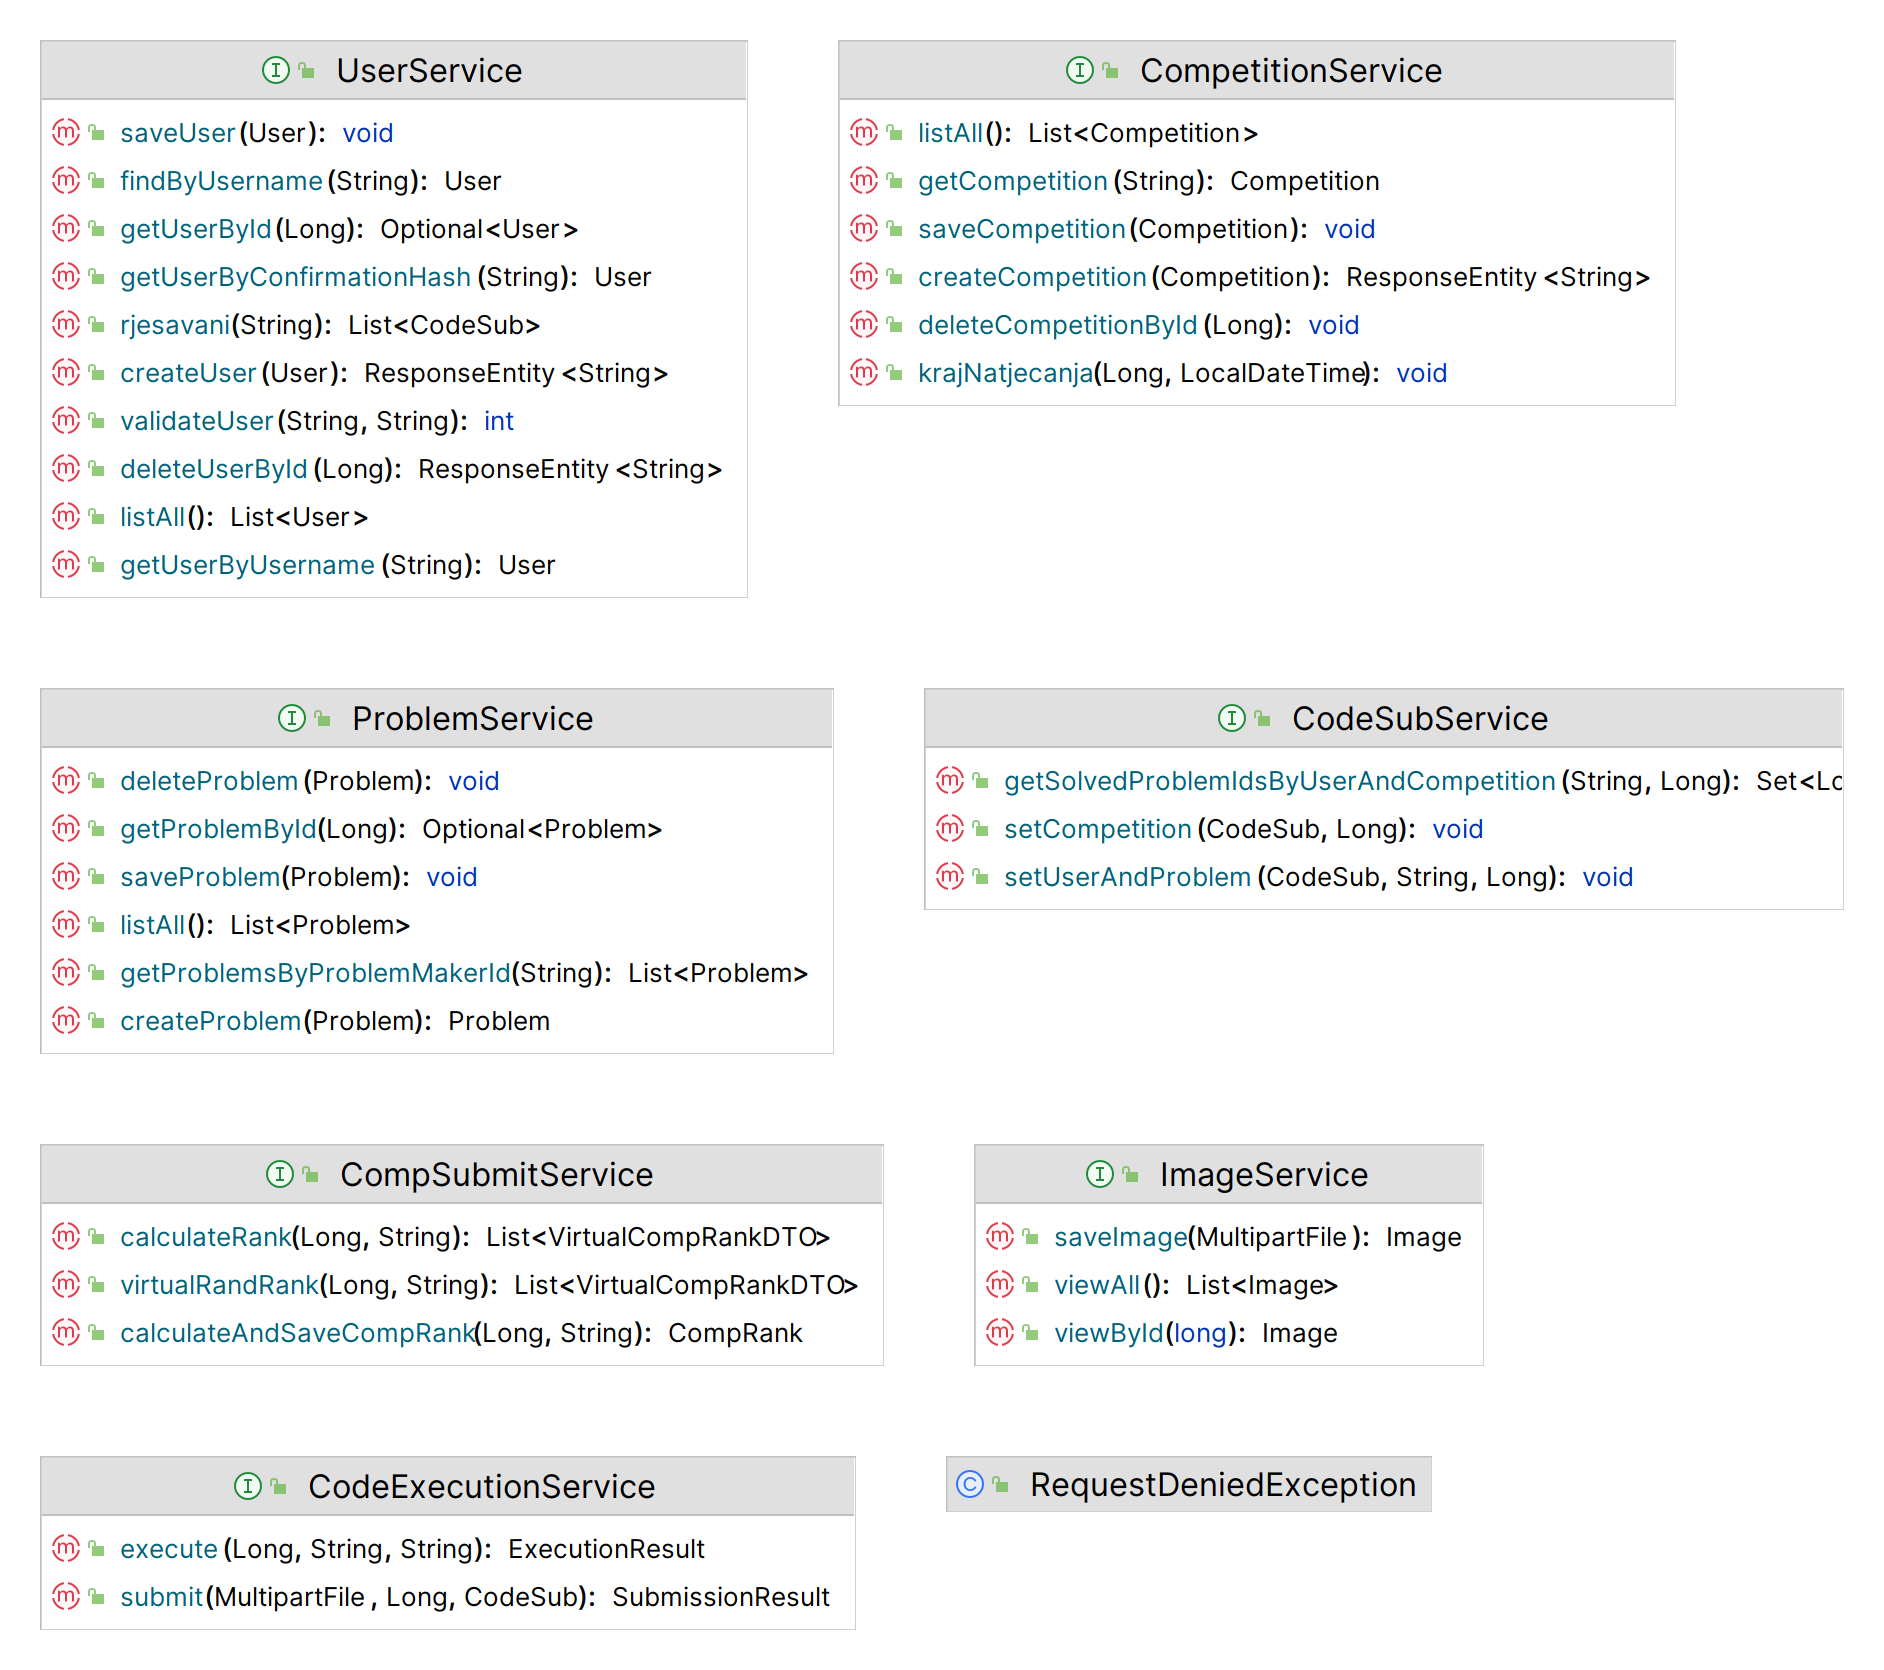
\includegraphics[width=\textwidth]{slike/services}
				\caption{Dijagram razreda: razredi Service}
					\label{fig:dr}
			\end{minipage}
			\end{figure}
					
			\eject
		
		\section{Dijagram stanja}
		
		\noindent{	
		UML-dijagram stanja je ponašajni UML-dijagram kojim se prikazuje
		diskretno ponašanje objekta ili sustava putem prelazaka između konačnog broja stanja, a često se za cjelokupni model stanja i prijelaza između stanja koristi izraz stroj stanja. Ova vrsta dijagrama se koristi za modeliranje ponašanja entiteta tijekom vremena, naglašavajući odgovor na dogadaje i okidače. Na dijagramu stanja, slika \ref{fig:dijagramstanja} prikazane su sve funkcionalnosti kojima natjecatelj može pristupiti.\\
		
		Proces kreće prijavom korisnika ulogom natjecatelja. Na početnoj stranici natjecatelj može pristupiti aktivnom natjecanju, otići na kalendar natjecanja, pregled profila korisnika, stranicu za vježbu ili stranicu s rezultatima. U bilo kojem slučaju korisnik može doći u stanje "Početna stranica", "Kalendar natjecanja", "Korisnici", "Vježba", "Rezultati". Iz svih se stanja može odjaviti.\\
		
		Odabirom kalendara stranica preusmjerava na kalendar s prikazanim natjecanjima, ukoliko su aktivni. U slučaju aktivnog natjecanja, natjecatelj može pristupiti natjecanju odabirom gumba "Pokreni natjecanje". Tim odabirom javlja se poruka upozorenja koja naglašava kako se korisnik ne bi smio koristiti nedopuštenim sredstvima. Odabirom gumba "Pokreni natjecanje", natjecanje se aktivira te počinje odbrojavanje vremena. Korisnik može vidjeti tekst svakog zadatka, preći na sljedeći zadatak, testirati rješenje, učitati svoj kod te završiti natjecanje. Završetkom natjecanja natjecatelj vidi rang listu svih natjecatelja koji su pristupili tom natjecanju na stranici rezultati.\\
		
		Odabirom poveznice Korisnici, stranica prikazuje profile svih registriranih korisnika (potvrđenih od administratora). Klikom na bilo kojeg korisnika prikazuju se podatci o njegovom profilu. Za natjecatelja se prikazuju podatci o broju točno riješenih zadataka, broju isprobanih zadataka te su za sva natjecanja na kojima je imao dobar plasman iscrtani pehari. S druge strane, profili voditelja sadrže popis učitanih zadataka s mogućnošću sortiranja i kalendar s popisom objavljenih natjecanja. Odabirom na zadatak pojedinog voditelja, moguće je vidjeti i riješiti taj zadatak.\\
		
		Odabirom poveznice Vježba stranica nudi dva načina vježbe: Virtualno natjecanje i Zadatci za vježbu. Odabirom zadataka za vježbu prikazuju se javno objavljeni zadatci svih voditelja. Klikom na ime zadatka ili na gumb Riješi započinje odbrojavanje vremena te natjecatelj može pokušati riješiti zadatak i testirati točnost svog koda. Odabirom virtualnog natjecanja stranica nudi dvije opcije: odabir pošlog natjecanja ili nasumično generiranog natjecanja. U slučaju nasumično generiranog natjecanja stranica poručuje kako je vrijeme ograničeno te klikom na pokreni natjecanje, natjecatelj započinje natjecanje. Odabirom prošlog natjecanja, prikazuje se kalendar u kojem korisnik može odabrati prijašnje natjecanje. Postupak provedbe natjecanja za oba slucaja virtualnog natjecanja je isti kao i za normalno natjecanje.\\ 
		Proces završava odjavom natjecatelja. 	
		}\\
		\begin{figure}[H]
			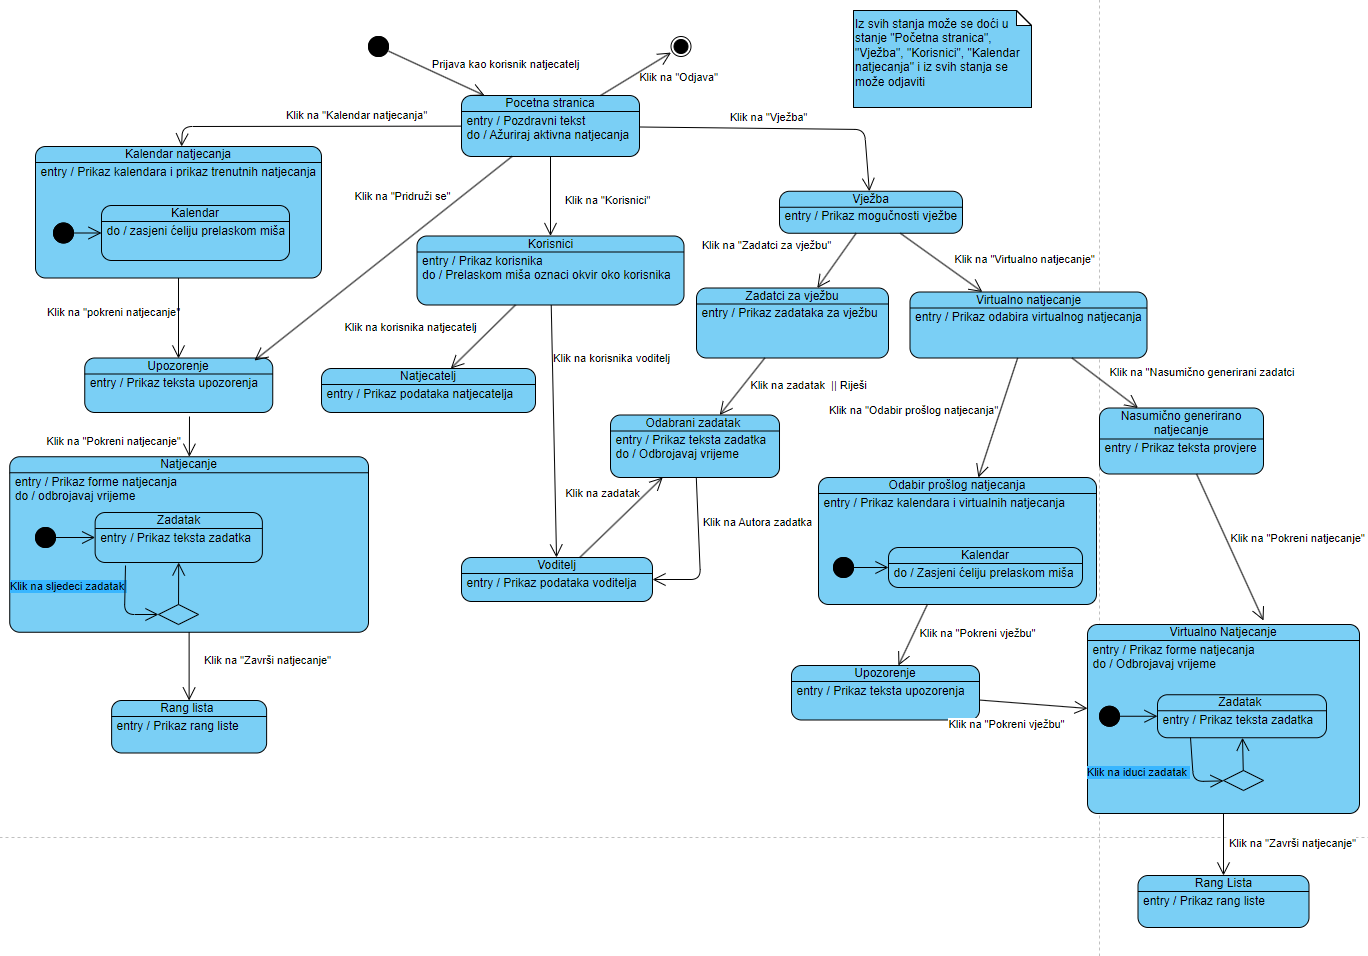
\includegraphics[scale=0.35]{slike/dijagram stanja}
			%veličina slike u odnosu na originalnu datoteku i pozicija slike
			\centering
			\caption{Dijagram stanja}
			\label{fig:dijagramstanja}
		\end{figure}	 
		
		\section{Dijagram aktivnosti}
		
		\noindent{

			Dijagram aktivnosti je vrsta UML-dijagrama koja se u programskom inženjerstvu koristi za modeliranje i grafički prikaz dinamičkog ponašanja sustava. Na njemu se prikazuje izvođenje aktivnosti kroz niz akcija koje čine upravljačke tokove i tokove objekata, s naglaskom na slijed i uvjete toka. Na dijagramu aktivnosti (slika \ref{fig:dijagramaktivnosti}) prikazan je proces kojim voditelj stvara zadatak za vježbu ili natjecanje.
			
			Proces započinje prijavom korisnika u sustav kao voditelj. Na početnoj stranici, klikom na "Kreiraj sadržaj", web aplikacija prikazuje 2 moguća odabira: kreiranje zadatka ili kreiranje natjecanja. Voditelj odabire što želi kreirati, te nakon odabira web aplikacija prikazuje formu za unos potrebnih podataka. Forma za stvaranje zadataka razlikuje se od forme za kreiranje natjecanja, ali bez obzira na odabrano, web aplikacija izvršava isti postupak.
			
			Nakon što voditelj klikne na gumb Izradi, web aplikacija provjerava jesu li uneseni svi podaci. Ako nisu, web aplikacija ne dopušta stvaranje te javlja voditelju da mora dopuniti izostavljene podatke. Kada su svi podaci uneseni, web aplikacija sprema kreirani sadržaj u bazu podataka te preusmjerava korisnika na drugu stranicu.  
		}\\
		
			
		\begin{figure}[H]
			\includegraphics[scale=0.5]{slike/dijagram aktivnosti}
			%veličina slike u odnosu na originalnu datoteku i pozicija slike
			\centering
			\caption{Dijagram aktivnosti}
			\label{fig:dijagramaktivnosti}
		\end{figure}
			
			\eject
		\section{Dijagram komponenti}
		
		\noindent{
			UML-dijagrami komponenti su vrsta strukturnih UML-dijagrama koji prikazuju organizaciju i odnose komponenti koji čine programsku potporu. Pružaju vizualni prikaz arhitekture sustava, naglašavajući modularnu strukturu i interakcije između komponenti. Dijagram komponenti na slici \ref{fig:dijagramkomp} opisuje organizaciju i međuovisnost
			komponenti, interne strukture i odnose prema okolini. 
			
			U web aplikaciji BytePit postoje dvije velike komponente: Frontend - React i Backend - Spring Boot. Te dvije komponente komuniciraju preko sučelja REST\_API koje je zaduženo za komunikaciju frontend dijela aplikacije s backend dijelom aplikacije. U React komponenti sučelje REST\_API spaja se na komponentu React view koja komunicira s ostalim Frontend komponentama. Sve frontend komponente ovise o komponenti ReactJS koja je zadužena za dohvaćanje React biblioteka. S druge strane, u komponenti Spring Boot REST\_API je spojeno na komponentu Rest Controller koji je glavna komponenta za backend dio aplikacije. Sučelje JPA s vezom "ball and soccet" povezuje komponente Repository i JPA repository, JPA repository omogućuje komunikaciju s bazom podataka. Web aplikacija se spaja na vanjske komponente: web preglednik preko sučelja HTTP\_Request koji podržava HTTP protokol i sve njegove operacije (Get, Post, Put, Delete), također na bazu podataka preko sučelja postgreSQL.
		
			\begin{figure}[H]
				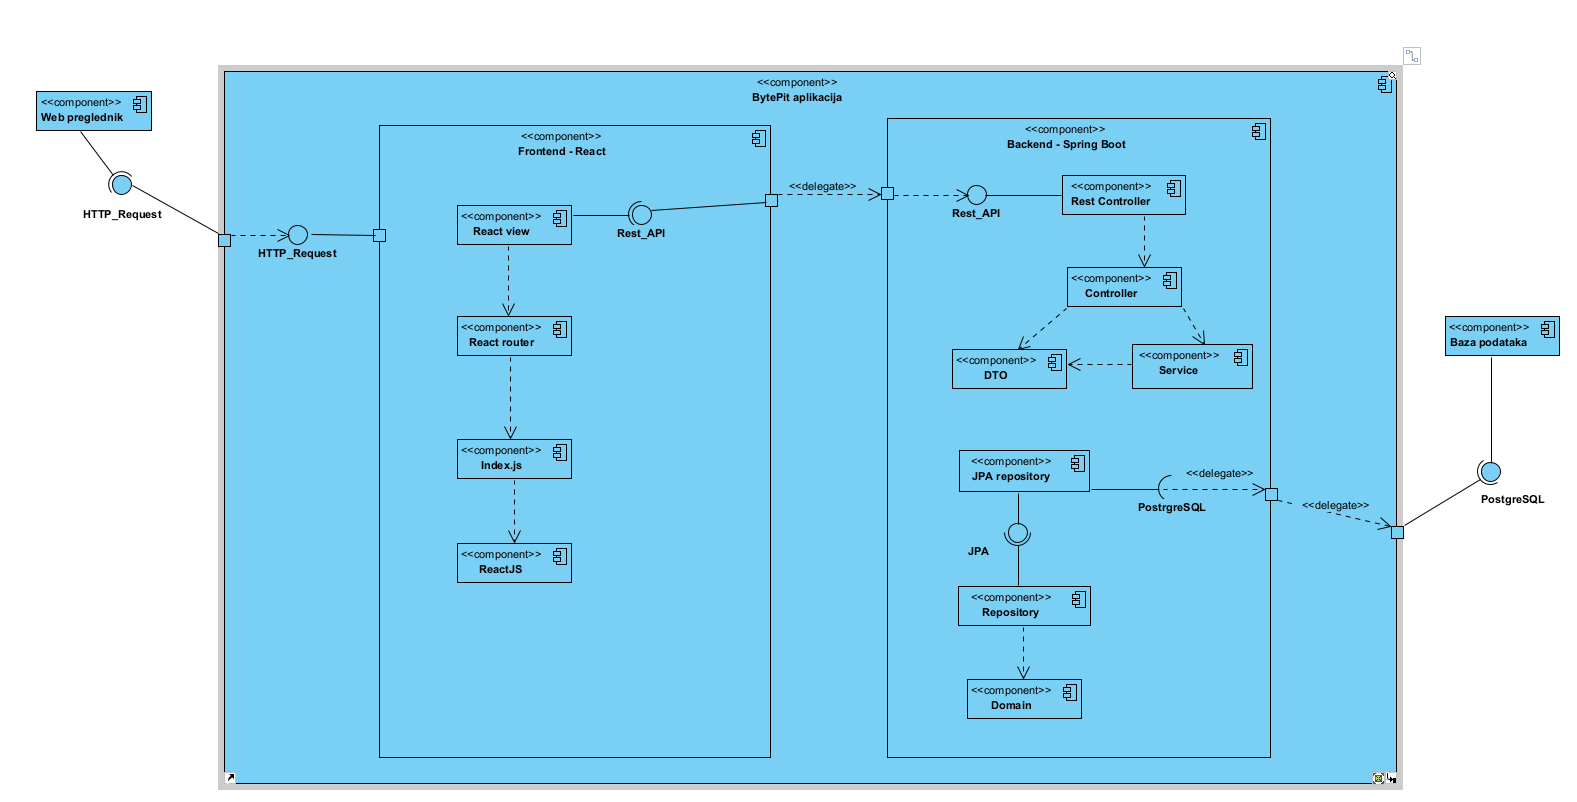
\includegraphics[scale=0.4]{slike/Dijagram komponenti}
				%veličina slike u odnosu na originalnu datoteku i pozicija slike
				\centering
				\caption{Dijagram komponenti}
				\label{fig:dijagramkomp}
			\end{figure}